\documentclass[conference,final]{IEEEtran}

\usepackage{latex8}
\usepackage{times}

\usepackage[utf8]{inputenc}
\usepackage{graphicx}
\usepackage{url}
\usepackage{float}
\usepackage{times}    
\usepackage{multirow}    
\usepackage{listings}   
\usepackage{times}     
\usepackage{paralist}    
\usepackage{wrapfig}    
\usepackage[small,it]{caption}
\usepackage{multirow}
\usepackage{ifpdf}
\usepackage{srcltx}


\usepackage{listings}
\usepackage{keyval}  
\usepackage{color}
\definecolor{listinggray}{gray}{0.95}
\definecolor{darkgray}{gray}{0.7}
\definecolor{commentgreen}{rgb}{0, 0.4, 0}
\definecolor{darkblue}{rgb}{0, 0, 0.4}
\definecolor{middleblue}{rgb}{0, 0, 0.7}
\definecolor{darkred}{rgb}{0.4, 0, 0}
\definecolor{brown}{rgb}{0.5, 0.5, 0}

\lstdefinestyle{myListing}{
  frame=single,   
  backgroundcolor=\color{listinggray},  
  %float=t,
  language=C,       
  basicstyle=\ttfamily \footnotesize,
  breakautoindent=true,
  breaklines=true
  tabsize=2,
  captionpos=b,  
  aboveskip=0em,
  belowskip=-2em,
  %numbers=left, 
  %numberstyle=\tiny
}      

\lstdefinestyle{myPythonListing}{
  frame=single,   
  backgroundcolor=\color{listinggray},  
  %float=t,
  language=Python,       
  basicstyle=\ttfamily \footnotesize,
  breakautoindent=true,
  breaklines=true
  tabsize=2,
  captionpos=b,  
  %numbers=left, 
  %numberstyle=\tiny
}

\newcommand{\up}{\vspace*{-1em}}
\newcommand{\upp}{\vspace*{-0.5em}}
\newcommand{\numrep}{8 }
\newcommand{\samplenum}{4 }
\newcommand{\tmax}{$T_{max}$ }
\newcommand{\tc}{$T_{C}$ }
\newcommand{\bj}{BigJob}

% \title{Running Molecular Dynamics Ensembles and Replica-Exchange
%   Simulations on Azure} 
%\title{Patterns for Pleasingly Parallel Bio-molecular Simulations on
%Azure}

\title{Abstractions for Loosely-Coupled and Ensemble-based Simulations
  on Azure}

\author{
Andr\'e Luckow$^{1}$, Shantenu Jha$^{1,2,3,*}$\\
  \small{\emph{$^{1}$Center for Computation \& Technology, Louisiana State University, USA}}\\
  \small{\emph{$^{2}$Department of Computer Science, Louisiana State University, USA}}\\
  \small{\emph{$^{3}$e-Science Institute, Edinburgh, UK}}\\
  \small{\emph{$^{*}$Contact Author: \texttt{sjha@cct.lsu.edu}}}\\
}

%\date{}

\def\acknowledgementname{Acknowledgements}
\newenvironment{acknowledgement}%
{\section*{\acknowledgementname}%
\parindent=0pt%
}

\newif\ifdraft
\drafttrue
\ifdraft
\newcommand{\llnote}[1]{ {\textcolor{green} { ***JK: #1 }}}
\newcommand{\alnote}[1]{ {\textcolor{blue} { ***AL: #1 }}}
\newcommand{\jhanote}[1]{ {\textcolor{red} { ***SJ: #1 }}}
\else
\newcommand{\llnote}[1]{}
\newcommand{\alnote}[1]{}
\newcommand{\jhanote}[1]{}
\fi

\begin{document} 

\maketitle    

\begin{abstract}
  \jhanote{I guess we should have one, even if this is a 4page paper}
\end{abstract}

\section{Introduction}
\up
% Distributed infrastructures have been used by many applications to
% advance understanding in their disciplines. Clouds as represented by
% Microsoft’s Azure Platform are emerging as an important class of
% distributed computational resources, for both data-intensive and
% compute-intensive applications. 

In spite of the promise of Clouds as a viable platform for Science \&
Engineering (SEA) applications, many fundamental persist about how
scientific applications will utilize clouds as presented, both now and
into the future? Many existing legacy applications no doubt will adapt
and take advantage of new capabilities, but it is unclear how clouds
as currently presented are likely to change (fundamentally?)  the
development and deployment of scientific applications, and the process
of scientific investigation. The challenges surrounding the effective
uptake of clouds are both broad and deep, in that, there are both
application-level questions as well as system-level questions. For
example, what kind of CI do clouds present, and how should clouds be
provisioned and what services should be provided to the scientific
community? The aim of this paper is to
explore... \jhanote{integrate..fill...} Emerging Cloud platforms such
as Azure, particularly arises as a consequence of the novelty and
relative simplicity of the cloud operating environment – resource
management, capacity planning capabilities, software environment \&
control etc.
 
% Cloud are posed to have a broad impact on scientific applications, as
% they provide novel and exciting opportunities for Science \&
% Engineering Applications (SEA). 

% how clouds -- particularly the Azure platform -- can support
% scientific applications in the domain of molecular dynamics.

Ensemble-based (enMD) approaches are commonly used in simulations to
facilitate drug discovery and to provide fundamental insight into
molecular structure, dynamics and interactions.  Different kinds of
ensemble-based approaches are commonly deployed: Ensembles of
independent simulations aim to improve the statistic significance of
MD simulations; % by simply performing the same simulation repeatedly
% (enD).  
%More demanding are ensembles of coupled simulations: 
in some scenarios, sampling of physical-states can be improved by the
infrequent attempt to exchange partial or complete simulation state
between a pair of replicas. The replica-exchange (RE)
algorithm~\cite{hansmann} is a well-known example of this class. In
spite of the exchange attempts, the coupling is small (a few state
variables are typically exchanged) and loose (not frequent).

In Luckow et\,al.~\cite{repex_ptrs} although efficient scale-out of RE
simulation was established, all resources utilized were TeraGrid
resources. We utilize the BigJob framework to decouple workload
submission from resource assignment; this results in a flexible
execution model, which in turn enables the distributed scale-out of
applications on multiple and possibly heterogeneous resources.
In~\cite{10.1109/CCGRID.2010.91} we extended this work to support
production grid infrastructures based on Condor as well as EC2-style
clouds (such as the FutureGrid).
 
% This is not a research paper, but an experience and experiment
% paper. 
The primary aim of this paper is to explore the abstractions that
Windows Azure platform provides and to determine how well established
abstractions for distributed computing can be extended to Azure.
% Based upon our research choose as our with respect to the enMD and
% REMD use case.
\jhanote{Given that we're not using SAGA BigJob here, should we call
  this an extension of the earlier work?}  We analyze the suitability
of the different abstraction provided by the Azure platform, such as
the AQS, ABS and the Worker Role API; we find that they provide
powerful tools for orchestrating distributed workloads, as found in
ensemble-based bio-molecular simulations.
% We show that Azure abstractions, such as the Azure Queue and ABS as
% well as the Worker Role API, provide powerful tools for orchestrating
% distributed workload as found in the RE use case. 
We propose the BigJob API as a novel abstraction for managing a group
of Azure worker roles and for remotely executing sub-jobs on them. The
proposed framework will encapsulate Azure specifics so that the REMD
and enMD use cases can easily ported to Azure.  \jhanote{Should we
  propose BigJob as an additional abstraction for Azure?}
\alnote{rephrased paragraphe}\jhanote{Yes, reads better now. Tweaked a
  bit upstream in this paragraph too.}

This paper is structured as follows: In section~\ref{sec:azure} we
present an overview of the Azure platform and analyse the abstractions
provided it. The BigJob framework that provides the basis for the
Azure-based RE application is presented in
section~\ref{sec:bigjob-saga}. In section~\ref{sec:enMD-REMD} we
discuss the architecture of the Azure-based enMD and RE application.
A significant issue in cloud computing is performance. We provide an
in-depth performance analysis in section~\ref{sec:performance}.


\alnote{old notes:
\begin{itemize}
    \item Bio-ensembles on Azure and hybrid Grid/Clouds
    \item Amazon Cluster Compute benchmark
    \item Synchronous ARepex
    \item Fluctuation of runtime on the different VMs (set case for an
      asynchronous algorithm)
    \item Performance/cost as metric and argument
\end{itemize}}


\section{Related Work}
\up \alnote{Do we need related work? Or are our references
  sufficient?}  AzureBlast~\cite{azure_blast} \jhanote{I think
  references are good enough. I don't know if there is a
  protocol/space-economics of a 4page paper..}

\section{Windows Azure}
\label{sec:azure}
\up
Azure provides different higher level services, e.\,g.\ the Azure
AppFabric or Azure Storage, that can be accessed via HTTP/REST from
anywhere. Windows Azure offers a platform for on-demand computing and
for hosting generic server-side applications. The so-called Azure
fabric controller automatically monitors alls VMs, automatically
reacts to hardware and software failures and manages application
upgrades.

\subsubsection{Compute}

Windows Azure formalizes different types of virtual machines into
so called roles. Web roles e.\,g.\ are used to host web applications
and frontend code, while worker roles are well suited for background
processing. While these roles target specific scenarios, they are also
highly customizable. Worker roles can e.\,g.\ run native code. The
application must solely implemented a defined entry point, which is
then called by Azure. The Azure fabric controller automatically
manages and monitors applications, handles hardware and software
failures as well as updates to the operating system or to the
application.  Commonly, scientific applications utilize worker roles
for compute- and data-intensive tasks. AzureBlast~\cite{azure_blast}
e.\,g.\ heavily relies on worker roles for computing bio-sequences.

\subsubsection{Storage}

For storing large amounts of data the Azure storage platform provides
three key services: the \emph{Azure Blob Storage} (ABS) for storing large
objects of raw data, the \emph{Azure Table Storage} for
semi-structured data and the \emph{Azure Queue Storage} (AQS) for
implementing message queues.  The data is storage replicated across
multiple data centers to protect it against hardware and software
failures. In contrast to other cloud offerings (e.\,g.\ Amazon S3) the
Azure Storage Services provide strong consistency guarantees, i.\,e.\
all changes are immediately visible to all future calls. While
eventual consistency as implemented by S3~\cite{1294281} usually
offers a better performance and scalability, it has some disadvantages
mainly caused by the fact that the complexity is moved to the
application space.

ABS can store file up to a size of 1\,TB, which makes it
particularly well suited for data-intensive application. The Amazon S3
service e.\,g.\ restricts the maximum file size to 5\,GB. Further, the
access to the ABS blob storage can be optimized for certain usage modes:
\emph{block blob} can be split into chunks which can be uploaded and
downloaded separately and in parallel.  Thus, block blobs are well
suited for uploading and streaming large amounts of data. \emph{Page
  blob} manage the storage as an array of pages. Each of these pages
can be addressed individually, which makes page blobs a good tool for
random read/write scenarios. \emph{Azure XDrive} provides a durable
NTFS volume, which is backed by a page blob. In particular legacy
applications that heavily utilize file-based storage can simply be
ported to Azure using XDrive.

The AQS provides a reliable storage for the delivery
of messages within distributed applications.  The queue service is
ideal to orchestrate the various components of a distributed
applications, e.\,g.\ by distributing work packages or collecting
results, which could be running on Azure or on another resource,
e.\,g.\ a science cloud.

The Azure Table Storage is ideally suited for storing structured
data. Unlike traditional relational database systems, the table
storage is designed with respect to scale-out, low cost and high
performance similar to Google's BigTable~\cite{bigtable2006}
system. For legacy application Azure also provides a SQL-Server based,
relational datastores called SQL Azure. In contrast to Azure tables,
SQL storage supports common relation database features, such as
foreign keys, joins and SQL as query language.


\section{Azure BigJob}
\label{sec:bigjob-saga}
\up
\emph{BigJob} is a SAGA-based Pilot-Job implementation. SAGA~\cite{saga_url} 
is a simple, POSIX-style API to the most common distributed functions, which 
is a sufficiently high-level of abstraction so as to be 
independent of the diverse and dynamic Grid environments. 
In contrast to other Pilot-Job implementations, e.\,g.\ Falkon, BigJob can
natively works independent of the underlying distributed infrastructure across different
heterogeneous backend, e.\,g.\ Grids and Cloud, reflecting the
advantage of using a SAGA-based approach. Further, the framework is
extensible and provides several hooks that can be used to support
other resource types and Pilot-Job frameworks.

As shown in Figure~\ref{fig:figures_distributed_pilot_job}, BigJob 
provides a unified abstraction to Grids, Condor pools,
EC2-style Cloud as well as to the Windows Azure platform.
Using the same API, applications can dynamically allocate
resources via the big-job interface and bind sub-jobs to these
resources. 

\begin{figure}[t]
    \centering
        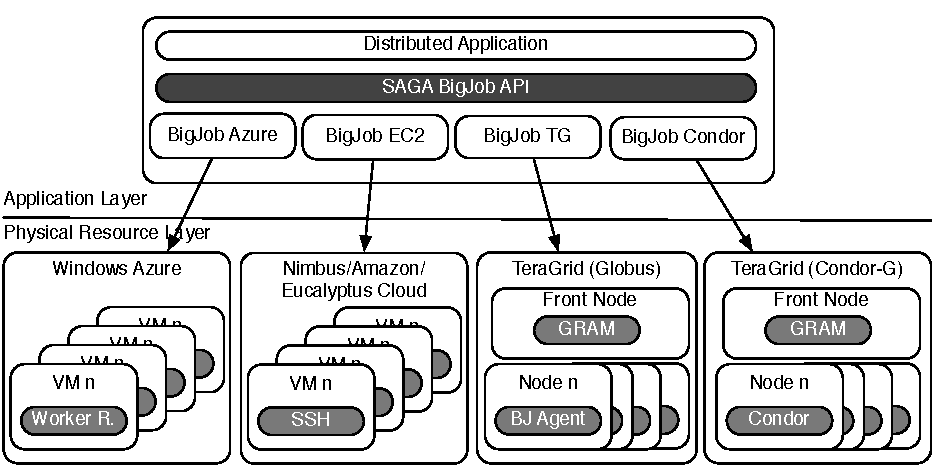
\includegraphics[width=0.45\textwidth]{figures/distributed_pilot_job}
        \caption{\textbf{Overview of the SAGA-based Pilot Job:} The
          SAGA Pilot Job API is currently implemented by four
          different backends - one for Grids, Condor and for
          EC2-style and Azure Clouds.\up}
    \label{fig:figures_distributed_pilot_job}
    \up
\end{figure}


% \begin{figure}[ht]
%     \centering
%     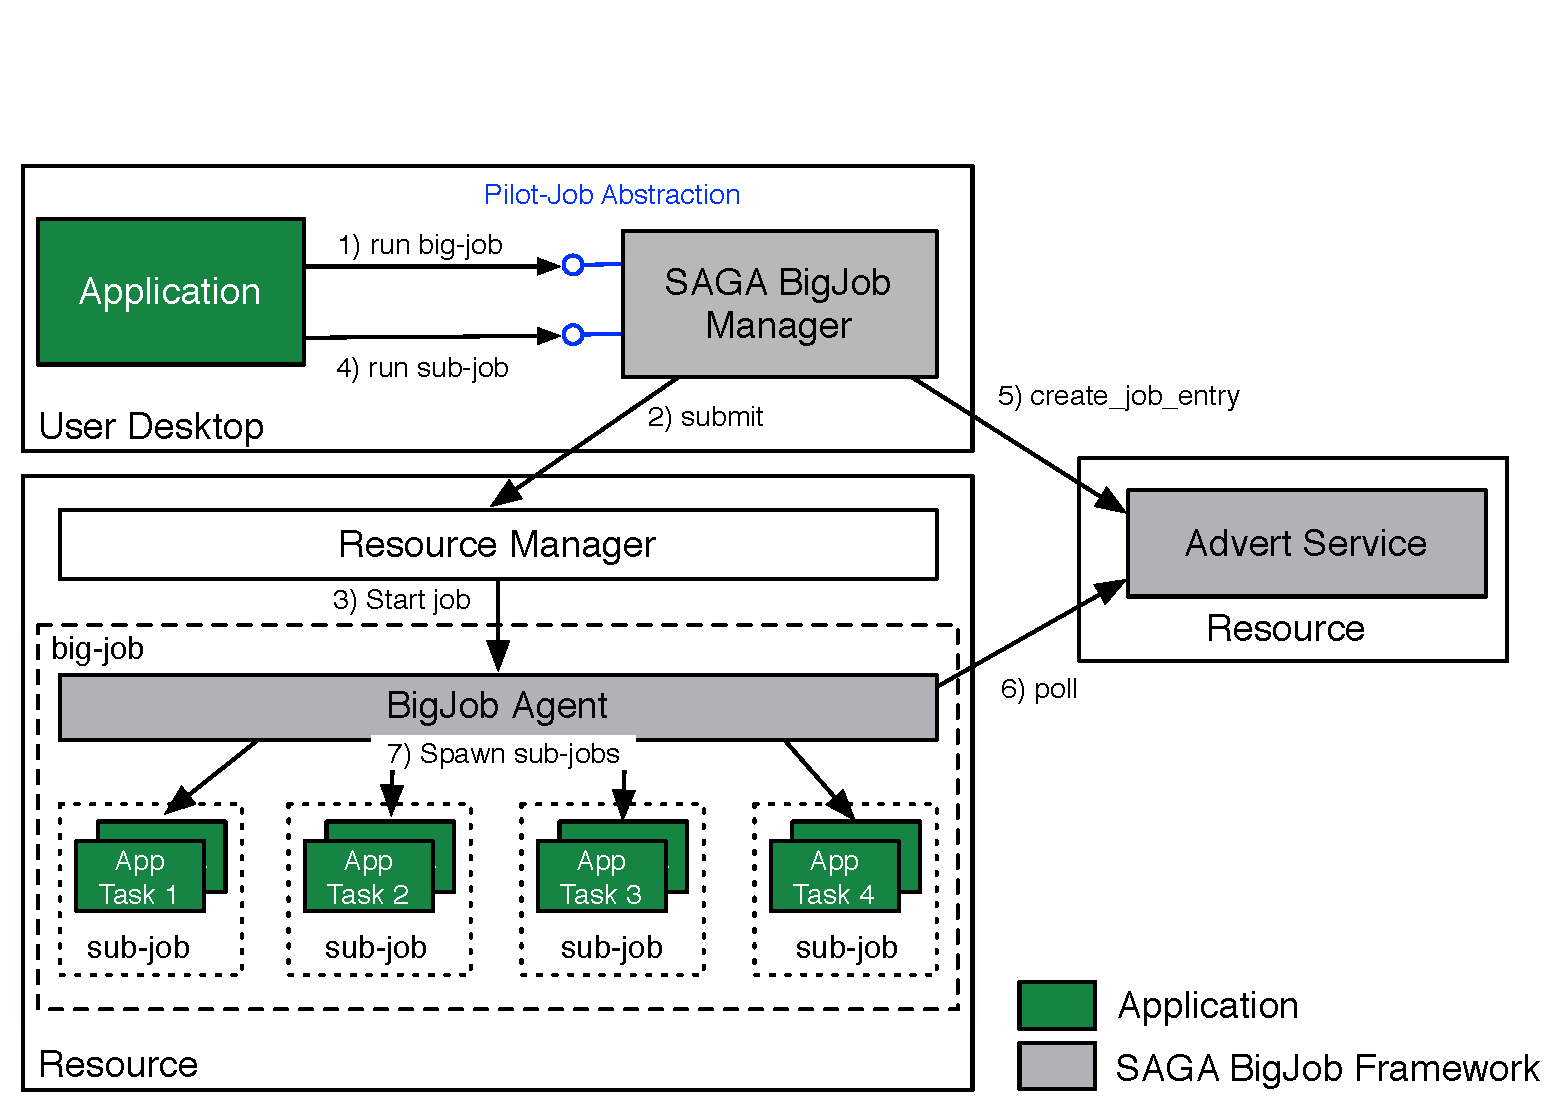
\includegraphics[width=0.45\textwidth]{figures/bigjob}
%    \caption{BigJob Architecture: The core of the framework, the
%       BigJob Manager, orchestrates a set of sub-jobs via a
%       BigJob Agent using the SAGA job and file APIs.  The
%       BigJob Agent is responsible for managing and monitoring sub-jobs.\up}
%    \label{fig:figures_bigjob}
%    \up
% \end{figure}
% Figure~\ref{fig:figures_bigjob} shows an overview of the SAGA BigJob
% implementation for computational Grids. The Grid BigJob comprises of
% three components: (i) the BigJob Manager (BM) that provides the Pilot-Job
% abstraction and manages the orchestration and scheduling of BigJobs
% (which in turn allows the management of both big-job objects and
% sub-jobs), (ii) the BigJob Agent that represents the pilot job.


Applications can utilize the framework via the big-job and sub-job
classes. Both interfaces are syntactically and semantically consistent
with the other SAGA APIs: a sub-job e.\,g.\ is described using 
the standard SAGA job description; job states are expressed
using the SAGA state model. Before running sub-jobs, an application must initialize
a big-job object. The BigJob Manager then queues a job,
which actually runs a BigJob Agent on the respective remote
resource. For this agent a specified number of resources is
requested. Subsequently, sub-jobs can be submitted through the BigJob
Manager using the job-id of the BigJob as reference. The BigJob
Manager ensures that sub-jobs are launched onto the correct
resource based upon the specified job-id using the right number of
processes. 

%%%%%%%%%%%%%%
\jhanote{I am a bit confused about if we're using BigJob-Azure in
  conjuction with other BigJob agents, i.e i.e., SAGA-BigJob API is
  used, but not SAGA in the execution?  Is this correct?}
\alnote{The Azure BigJob is completely self-contained and
has nothing in common with the SAGA BigJob except the API. Hope this gets
clearer once I remove the SAGA BigJob stuff.}

Figure~\ref{fig:figures_bigjob_azure} illustrates the architecture of
the Azure-based BigJob. Similarly, the BM is responsible for accepting
simulation requests from the end-user and for orchestrating the
sub-job runs.  In contrast, to the Grid BigJob, which heavily utilizes
different SAGA API, such as the job, file and advert APIs, the Azure
BigJob is built directly on top of the Azure APIs.

In the BM launches the BigJob Agents using the Azure Service
Management API.  The Service Management API is a RESTful HTTP API - as
part of this project we developed a Python library that can be used to
access this Azure capability~\cite{azure-service-python}. The BigJob
Agents run within Azure worker roles, which are the Azure abstraction
for compute-intensive background tasks. The agent itself is
implemented in C\#/.NET. Azure also enables users to run native code
within worker roles, i.\,e.\ the agent is able to execute existing
native molecular dynamic (MD) codes, e.\,g.\
NAMD~\cite{Phillips:2005gd} and AMBER~\cite{cheatham-5}.  Azure
currently does not support MPI computations across multiple worker
roles, thus each MD simulation is limited to 8 cores.


The BM creates work packages for each sub-job and distributes them 
to the agents using the AQS. The AQS provides 
the ideal abstraction for this purpose by offering a reliable and scalable 
way for delivering messages to distributed components. These can but do not
have to be hosted on Azure. The SAGA-based BigJob in contrast utilizes
the SAGA advert service, a central key/value store, for this purpose. 
For each new job, an advert entry is created by the BigJob Manager. 
The agent periodically polls for new jobs. Azure Queues provide a higher
level of abstractions ensuring atomicity and an at least once semantic.

%\begin{wrapfigure}{R}{0.4\textwidth}
\begin{figure}
    \centering
    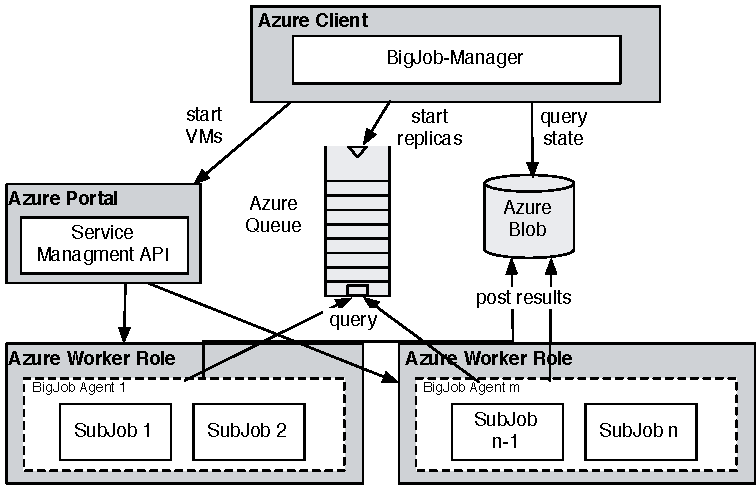
\includegraphics[width=.4\textwidth]{figures/bigjob_azure}
    \caption{\textbf{Azure-based BigJob:} The framework
      utilizes the queue storage for distributing work
      packages from the BigJob Manager to the
      BigJob agents running on multiple worker roles.}
    \label{fig:figures_bigjob_azure}
    \up
\end{figure}

Once the agents are started, they query the Azure queue for new work
items.  If a work item is found, a simulation task is started, e.\,g.\
by running the requested MD code with right parameters. The framework
supports both the staging of parameter files as well as of the
executable. Files are staged through the ABS, i.\,e.\ the manager
uploads the respective files to the storage and the agents downloads
them before the run.

The BigJob Azure supports the notion of Azure affinity groups, which
can be used to co-locate compute tasks and storage. This is
particularly useful for data-intensive tasks, e.\,g.\ MapReduce
application, which need to transfer large amounts of data to worker
roles. At the same time the BM can also orchestrate worker roles that
are distributed across multiple affinity groups.


% The worker roles running the BigJob agent are managed by the BigJob Manager using
% the Azure Service Management API. In the initial version we will
% support the automatic start and stop of hosted services. In the final
% version there will be a possibility to automatically deploy agent code
% without the need to pre-configuring the VMs. 


% \alnote{Kalman Filter option: we need to convey how we make decisions?
% we need to understand the various trade-offs}

\section{Ensemble and Replia-Exchange Simulations on Azure}
\label{sec:enMD-REMD}
\up
Based on the BigJob framework both the scenarios, i.\,e.\ the
independent ensemble enMD and the coupled ensemble REMD,
have been ported to Azure. NAMD is used to carry out MD simulations.
Both applications utilize the BigJob API to create pilot jobs
and subsequently to submit sub-jobs to these. When a pilot job is
created the BigJob framework initializes the requested number
of worker roles with the specified size using the defined 
Azure service package. The replicas themselves are submitted as
sub-job. The sub-jobs per worker role depends on the size of the worker role --
Azure currently supports worker roles up to 8 cores. In contrast
to other infrastructure types such as EC2 and the TeraGrid, MD jobs
cannot be spawned across multiple nodes. After the sub-job terminates,
the master can collect the result via the ABS. In the REMD
case the output is parsed to obtain the energy level of the replica. 
The Metropolis scheme~\cite{metropolis:1087} is used to determine whether
an exchange is conducted. Finally, a new generation of replicas is launched.

Both enMD and REMD can greatly benefit from the capabilities of Azure. If greater 
accuracy is required or a deadline must be met, it can 
seamlessly scale-out to more worker roles.  The
Azure fabric controller monitors all VMs running the worker roles and
automatically restarts the worker roles if necessary. Further, Azure
provides various kinds of reliable and scalable storage options to
express different coordination schemes, e.\,g.\ the master-worker
communication can be conducted via the described message queue.



\section{Performance Analysis}
\label{sec:performance}
\up
The aim of this section is not to perform detailed systematic
performance measures and analysis, but to illustrate the
representative usage modes BigJob can support, and to explain how they
are supported.  We discuss two scenarios that are representative of
how applications would typically use multiple distributed
infrastructures. We focus our attention on RE MD (REMD)
simulations and a workload as \numrep replicas of a Hepatitis-C virus
(HCV) model, each replica running for 500 timesteps.

\subsection{BigJob Startup Times} 
\up
Initially, we analyze the overheads resulting from the usage of BigJob across
different infrastructures. Typically, the main overhead when using
BigJob results from the queueing time at individual resources for
Grids and from the VM creation time for Cloud environments.
Figure~\ref{fig:performance_setup_time} compares the average startup times of
the different Pilot-Job backends for Grids, Condor pools and Clouds. Each 
experiment was repeated at least 10 times.

\begin{figure}[htbp]
    \centering
        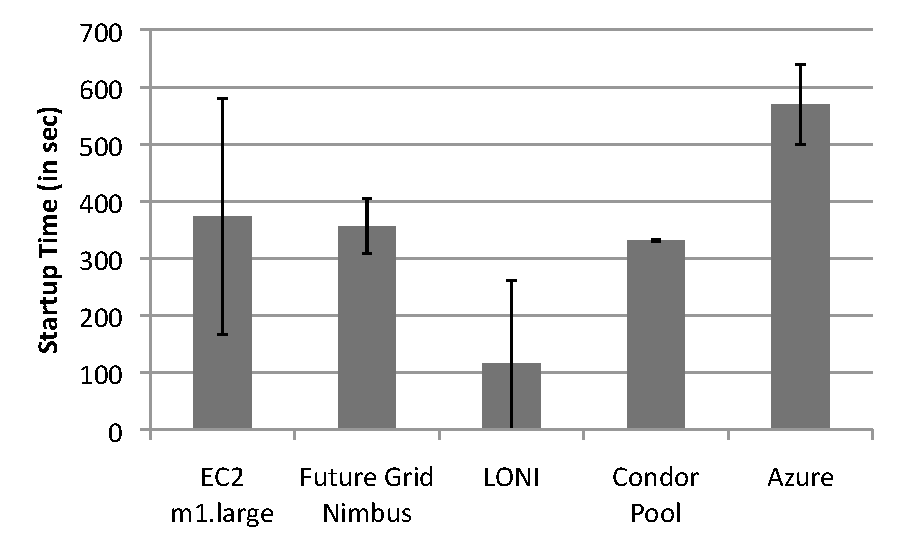
\includegraphics[width=0.46\textwidth]{performance/setup-times}
    \caption{\textbf{BigJob Startup Times:} In Grids the startup time
      greatly depends upon the queuing time at the local resource
      manager. However, in our experiments also Clouds showed a high
      fluctuation in the queueing time. Azure shows a slightly higher
      startup time than the science and the EC2 clouds.\up}
    \label{fig:performance_setup_time}
\end{figure}

Interestingly for the experiments conducted, the startup times for the
Cloud environments were observed to be larger than queue-waiting time
for the LONI resource Poseidon, which coincidentally was very lightly
loaded during the course of these experiments. Obviously, the startup
of a VM involves higher overheads than spawning a job on an already
running machine: a resource for the VM must be allocated, the VM must
be staged to the target and booted up. The following experiments will
also show that especially the already oversubscribed intra Cloud
network and thus, the staging of the VM can be a bottleneck. Azure VMs
showed with $>10$\,min the longest waiting time (about 200\,sec longer than EC2), which
is consistent Hill et\,al.~\cite{hill10}.  Further,
high fluctuations in the waiting times can be observed. These waiting time
usually correlate to the current load of the chosen data center, which again
depends on external factors, such as the location of the data center or 
the date/time of the request.

BigJob provides the possibility to manage a set of VM and removes the
need of the application to manage individual VMs. By utilizing
the different BigJob cloud and grid backends, fluctuation in the waiting 
times can be equalized. Further, BigJob provides the possibility
to dynamically add resources to an application, e.\,g.\ in case a
resource is heavily loaded and is showing long wait times.


% Also,
% there is a large fluctuation in particular in the EC2 environment
% probably caused by the fact that insufficient resources were available
% at certain times.

\subsection{Replica Ensembles on Different Resource Types}
\up
\label{sec:performance_namd}
\begin{figure}[htbp]
    \centering
        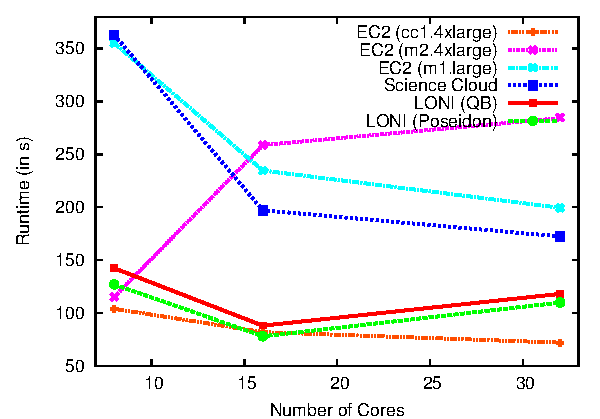
\includegraphics[width=0.46\textwidth]{performance/namd_run}
    \caption{\textbf{NAMD Runtimes on Different Resource Types: } The
          graph shows that the new EC2 cluster compute instances are 
          able to outperform other Cloud resources as well as traditional
          HPC resources as QB and Poseidon.}
    \label{fig:performance_namd_run}
    \up
\end{figure}

We run experiments in different Cloud environments: the Nimbus Science 
Cloud of the University of Chicago and the Amazon EC2 environment is used. In general, each Cloud has 
its characteristics. The Nimbus Cloud is accessed via the WSRF
interface, while for EC2 the Amazon command line client is used. 
Each Nimbus VM provides 2 virtual cores and 3.7\,GB memory. 
Amazon offeres different VM types with up to 8 cores. We used the largest 
VM type (m2.4xlarge) with 8 cores and 68.4\,GB of memory,
the m1.large instance type with 2 cores and 7.5\,GB  and the recently launched
cluster compute instances~\cite{ec2-cc}, which provide a pair of quad-core Intel 
X5570 (Nehalem) processors with 23\,GB memory. In contrast to other instance types,
cluster compute instances are connected using 10 Gbps Ethernet.


\begin{figure}[htbp]
    \centering
        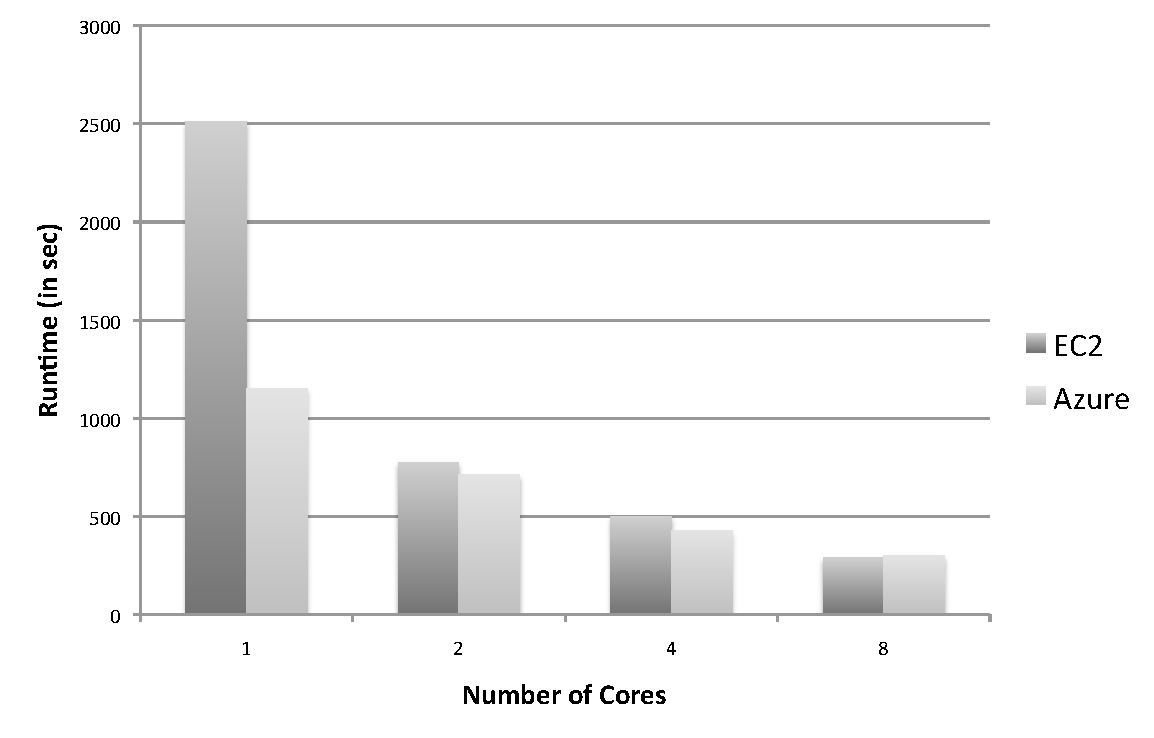
\includegraphics[width=0.46\textwidth]{performance/namd_ec2_azure.pdf}
    \caption{\textbf{NAMD Performance on Azure and EC2:} In particular on smaller VM sizes (1-4 cores) Azure 
    outperforms EC2. The 8 core EC2 VM cc1.xlarge shows a slightly better performance than the Azure 8 core VM,
    however at a higher cost (1.16\,\$ in comparison to 0.96\,\$).}
    \label{fig:performance_namd_ec2_azure}
    \up
\end{figure}

Figure~\ref{fig:performance_namd_ec2_azure} presents an performance 
benchmark consisting of a NAMD simulation run on Azure and on comparable 
EC2 resources. For this purpose, an EC2 instance type with a similar core
count and price is chosen. Azure outperforms EC2 Windows instances in 
most cases; which is in noteworthy, since the costs for 2, 4 and 8 core VMs are
drastically lower on Azure. Table~\ref{tbl:costs} summarizes the
costs of selected EC2 and Azure scenarios. In particular, the EC2
Linux instances show a good price/performance ratio. For Windows
instances Azure provides a favorable optimum.


% Since the underlying hardware is not known
% one can only speculate about the reason. Microsoft controls the
% hardware in its data center und optimizes its custom-built Azure
% Hypervisor with respect to this hardware~\cite{Krishnan:2010nx}, which
% could be a reason for the better performance. 

\begin{table}[ht]
	\begin{footnotesize}
		\begin{tabular}{|l|c|c|c|c|c|}
	        \hline
	        VM Type                 &CPU h  &\#Core &\#VM &\tc &Costs  \\ \hline
	        %EC2 m1.large  (Linux)   &2          &4     &355\,sec    &0.27\$  \\ \hline
	        EC2 m2.4xlarge (Lin)  &2.40\$  &8          &1      &128\,sec     &0.08\$ \\ \hline
	        EC2 cc1.4xlarge (Lin) &1.60\$  &8          &1      &45\,sec     &0.04\$ \\ \hline
	        EC2 c1.xlarge   (Win)   &1.16\$  &8          &1      &290\,sec    &0,09\$ \\ \hline
	        Azure XL (Win)  &0.96\$ &8          &1      &301\,sec    &0,08\$ \\ \hline
		\end{tabular}
	\end{footnotesize}
	\caption{EC2 vs. Azure Costs\label{tbl:costs}}
	\up
\end{table}

\subsection{Data-Management on Azure}
\up
Azure provides various options to distribute data and
compute. Users can either select one of the currently six data centers or 
specify a geographic region (i.\,e.\ US, Europe, Asia) for storing data and
conducting computation. Further, Azure offers so-called affinity groups, 
an abstractions that can be used to control the co-location of data/compute.

To evaluate the available bandwidths and storage options, we conducted
the following experiment: a 4.3GB file is stored in the Azure Blob
Storage in the ``Anywhere Europe'' region. This file is then
downloaded by worker roles with different configurations: ``Anywhere
US'', ``Anywhere Asia'', ``Anywhere Europe'', a worker role located in
the same data center and one in the same affinity group.

% \jhanote{How does 'same affinity group' differ from ``Anywhere
%   Europe-Anywhere Europe'' case?}\alnote{hopefully improved
%   description} \jhanote{Yes}

\begin{figure}[htbp]
    \centering
        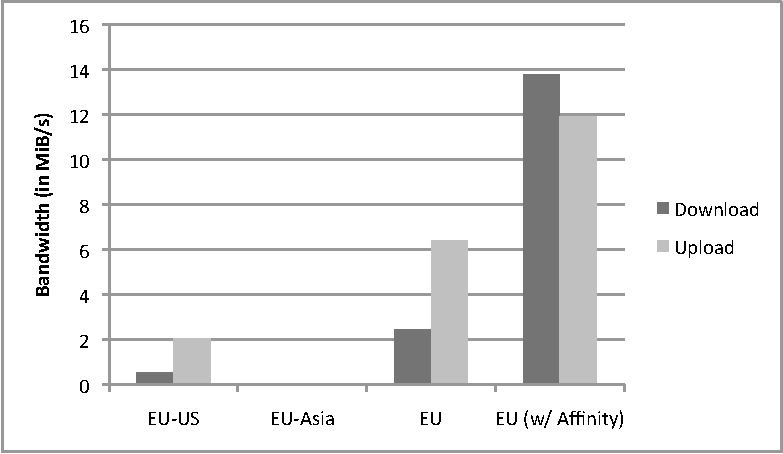
\includegraphics[width=0.46\textwidth]{performance/azure-data-transfer.pdf}
        \caption{\textbf{ABS Bandwidths Between
            Different Regions:} The achievable vary greatly with the
          distance between data and compute. Using affinity groups a
          bandwidth of approx. 12 MiB/s is achievable, which is
          comparable to the bandwidth that can be achieved by manually
          co-locating data and compute to the same data center.  }
    \label{fig:performance_azure-data-transfer}
    \up
\end{figure}
Figure~\ref{fig:performance_azure-data-transfer} shows the measured
bandwidths. Obviously, the further away the worker role, the smaller
the available bandwidth. Interestingly, even when staying in the same
region (``Anywhere Europe'') not the most optimal bandwidth could be
achieved. The best result (approx. 12 MiB/s) can be achieved when
placing worker roles and storage in the same data center or the 
same affinity group. While affinity groups provide a good abstraction
to manage the compute and storage location, the achievable bandwidths
are comparable to a manually placements of VMs and storage. That means 
that Azure does not provide an option to control data locality within
a data center.

While data locality is not critical for the EnMD and RE use case --
the Azure service package has a size of 8\,MByte -- for data-intensive
applications, such as MapReduce-based applications, this is an
important feature. By supporting the Azure affinities within the
BigJob framework, these requirements can be addressed.

\subsection{Replica-Exchange on Azure}
\up
\begin{figure}[htbp]
    \centering
        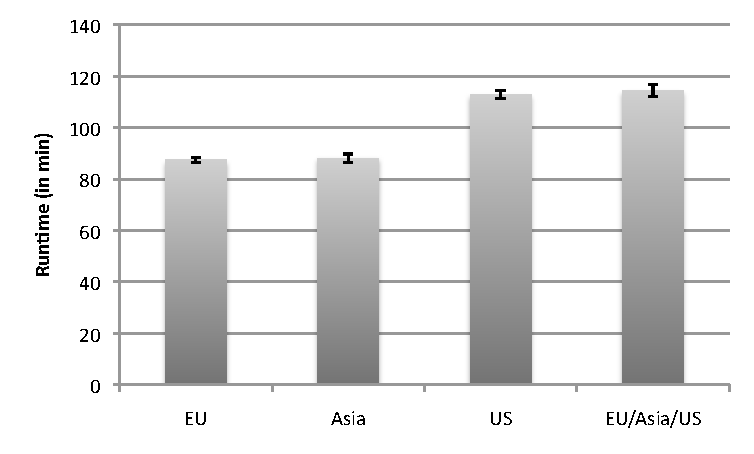
\includegraphics[width=0.46\textwidth]{performance/repex_runtime_per_region.pdf}
    \caption{\textbf{\tc for RE Run in Different Azure Regions:} Runtime for a RE simulation with 
    16 replicas each running on a small VM with 1 core for 500 timesteps and a total of 4 generations. The performance of
    the Azure fluctuates with the data center region. }
    \label{fig:performance_repex_runtime_per_region}
\end{figure}

Figure~\ref{fig:performance_repex_runtime_per_region} shows the
runtime of RE simulation with 16 replicas each running on a single
core VM for 500 NAMD timesteps. In total, we measured the time for 4
generations, i.\,e.\ for 64 attempted exchanges. As the graph shows
the runtime of this scenario fluctuates with the chosen Azure
region. The EU and Asia show a better performance than the US data
centers. BigJob also supports the distribution of sub-jobs across
multiple data centers. However, due to the coupling between the
replicas, the performance in this case depends on the slowest machine.

Figure~\ref{fig:performance_repex_scaleout_vmsizes} shows the runtime
of RE simulations with a different number of replicas on different VM
types. Again, each replica is run for 500 timesteps before an exchange
is attempted. The more replicas the higher the coordination overhead
at the master. As seen in the results, this overhead is hardly
observable.
\begin{figure}[ht]
    \centering
        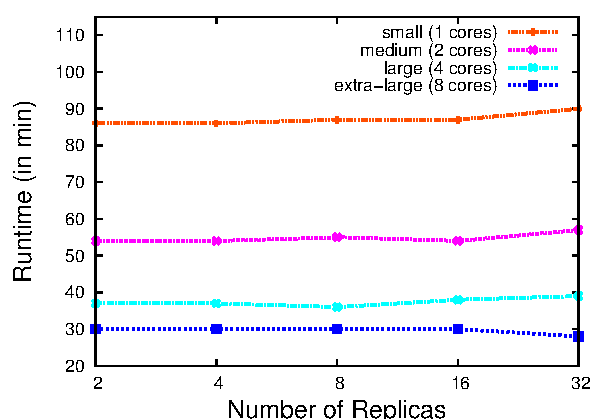
\includegraphics[width=0.46\textwidth]{performance/repex-azure.pdf}
    \caption{\textbf{\tc for Different VM Sizes and Number of Replicas:} With
    an increasing number of replicas a small coordination can be observed in most 
    scenarios. The chosen VM type has a great impact on the overall runtime. The larger
    the VM, the short \tc}
    \label{fig:performance_repex_scaleout_vmsizes}
\end{figure}

The chosen VM type greatly influences the overall runtime. Azure currently offers four
types of VMs: small VMs with 1 core, medium VMs with 2 cores, large VMs with 8 cores
and extra-large VMs with 8 cores. The larger the VM, the shorter the overall runtime.
However, the speedup from the 4 core to the 8 core VM is very small. 

Obviously, the best performance can be achieved on an extra-large
VM. The largest ensemble comprised of 32 replicas running on
extra-large VMs on a total of 256 cores.  With a runtime of
30\,minutes for the 16 replica case this setup is able to almost match
the performance of the TeraGrid resource QueenBee, where the same
scenario was executed in 26\,minutes (see~\cite{Luckow:2008fp} for
details).


\section{Conclusion and Future Directions}
\up
% RE is a popular algorithm often used by molecular dynamics approaches
% to enhance the sampling and rate of convergence for a biological
% system.

Ensemble-based MD simulations (enMD \& REMD) are commonly used
bio-molecular simulation approaches.%  to enhance the sampling and convergence for biomolecular
% simulations.
We have implemented the computational and coordination pattern
represented by RE to Azure, by extending the BigJob framework to
utilize the native abstractions provided by Azure, such as worker
roles, the Azure storage and affinity groups.
% including the underlying BigJob framework to Azure utilizing its
% native abstractions, such as worker
In contrast to other cloud offerings, Azure provides not only
bare-metal VMs to applications, but a managed PaaS environment for
running them. It also monitors and automatically restarts VMs and
applications if necessary. Further, it provides an integrated
development environment and a higher-level API, which simplifies the
development considerable in particular comparing to the efforts
necessary when running an application distributed across multiple
TeraGrid sites.  Using Azure we were able to achieve almost the same
sampling speed as on comparable Grid resources, such as QueenBee.

SAGA~\cite{saga_url} provides a simple, single interface to the common
distributed functionality (file/data, job/VM launch \& management
etc.), for a range of distributed cloud and grid infrastructure. SAGA
is heavily used by scientific applications for distributed
coordination – either fine grained as in MapReduce applications, or
coarse-grained as in the RE case.  Given this putative benefit, it
makes eminent sense to support Azure from within SAGA and to provide
SAGA adaptors to important Azure services.

Many scientific applications, e.\,g.\ DAG-based or MapReduce-based
application involve the management of large amounts of data. In the
future, we will further investigate different task placement
algorithms for data-intensive applications in conjunction with
different Azure worker roles, storage and affinity group setups.

\begin{acknowledgement} 
  \up \footnotesize{% Important funding for SAGA has been provided by
%     the UK EPSRC grant number GR/D0766171/1 (via OMII-UK) and HPCOPS
%     NSF-OCI 0710874.
    SJ acknowledges the e-Science Institute, Edinburgh for supporting
    the research theme. ``Distributed Programming Abstractions''%  and
%     theme members for shaping many important ideas. This work has also
%     been made possible thanks to the internal resources of the Center
%     for Computation \& Technology at Louisiana State University and
%     computer resources provided by LONI.
    We thank Joohyun Kim (CCT) for assistance with the RNA models. We
    thank FutureGrid and Microsoft for providing the cloud resources
    for the conducted experiments. }
\end{acknowledgement}

\up
\bibliographystyle{IEEEtran}
\bibliography{literatur,saga,cloud,repex}
\end{document}



